\documentclass[border=10pt]{standalone}
\usepackage{tikz}
\usetikzlibrary{automata, positioning, arrows.meta, calc}

\begin{document}
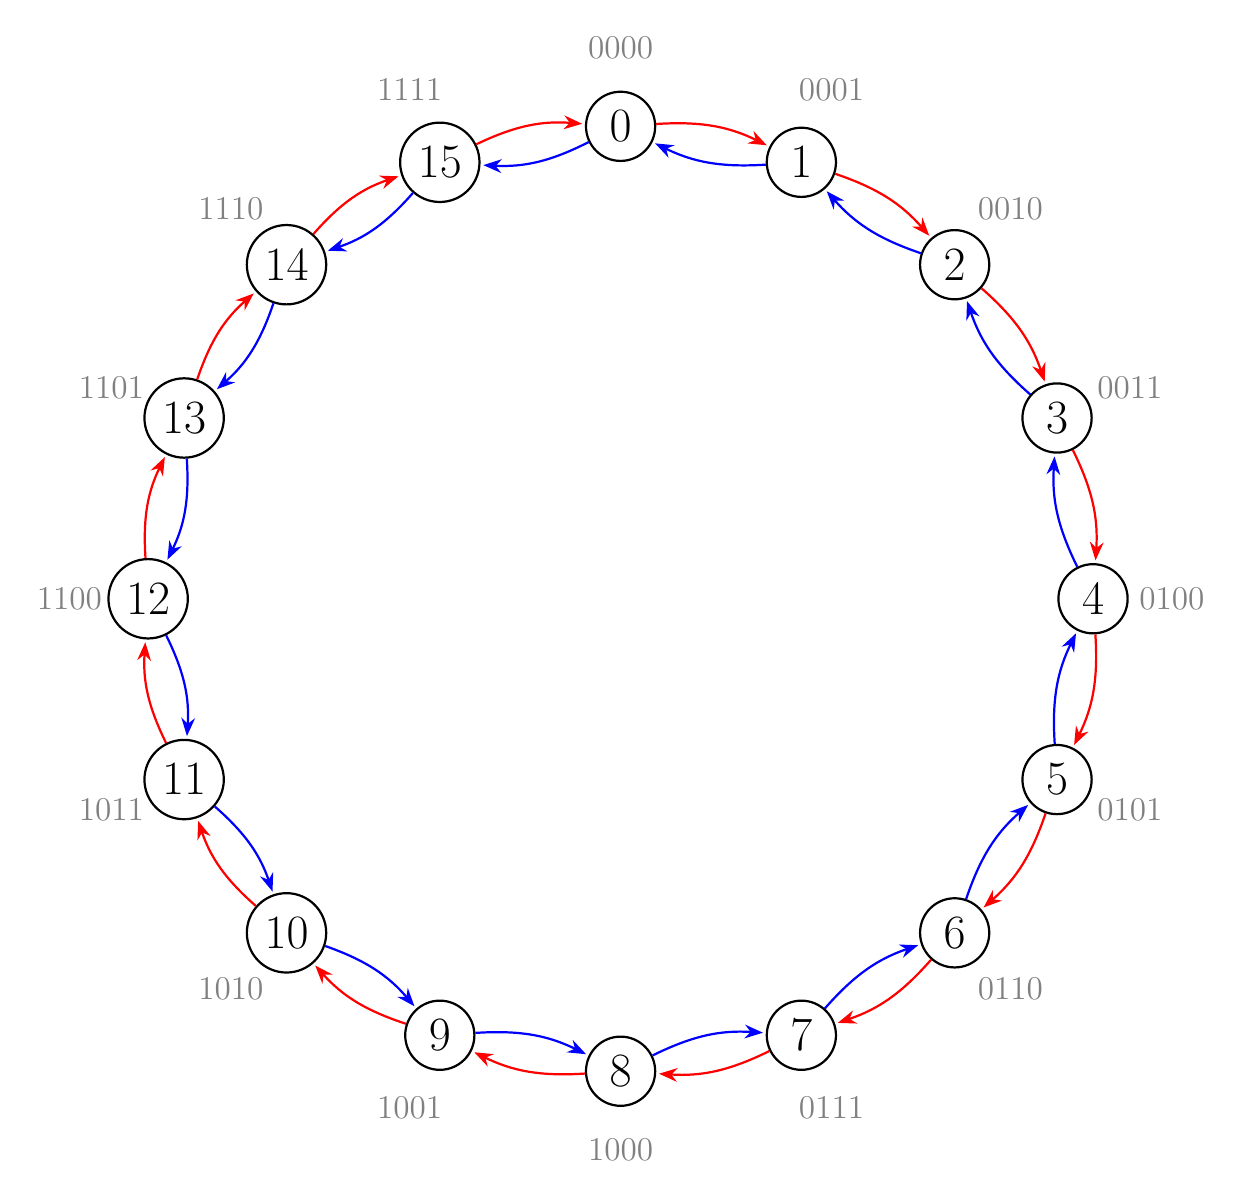
\begin{tikzpicture}[
    ->, >=Stealth, 
    shorten >=1pt, 
    auto, 
    node distance=2.5cm, 
    thick
]

    % Circular layout for states 0-15
    \def\radius{6.0cm}
    \def\n{16} % Number of states
    
    \foreach \i in {0,...,15} {
        % Angle: 90 degrees is top (0), clockwise is negative angle
        % 360/16 = 22.5 degrees per step
        % Start at 90 (Top) -> 0
        \pgfmathsetmacro{\angle}{90 - \i * 22.5}
        \node[state, font=\LARGE] (s\i) at (\angle:\radius) {\i};
    }
    
    % Transitions
    % UP Count (Clockwise, Red) - Inner Arcs or standard edges
    % DOWN Count (Counter-Clockwise, Blue) - Outer Arcs
    
    % Loop for edges
    \foreach \i in {0,...,15} {
        \pgfmathsetmacro{\next}{int(mod(\i+1,16))}
        \pgfmathsetmacro{\prev}{int(mod(\i-1+16,16))}
        
        % Up Count: i -> next
        \path[red] (s\i) edge [bend left=15] node[font=\small, text=red, swap] {} (s\next);
        
        % Down Count: i -> prev
        \path[blue] (s\i) edge [bend left=15] node[font=\small, text=blue, swap] {} (s\prev);
    }
    
    % Labels for Up/Down legend or annotation
    %\node[red, font=\Large] at (0, 1.0) {Up Count};
    %\node[blue, font=\Large] at (0, -1.0) {Down Count};
    
    % Binary Values
    \foreach \i/\bin in {
        0/0000, 1/0001, 2/0010, 3/0011, 
        4/0100, 5/0101, 6/0110, 7/0111, 
        8/1000, 9/1001, 10/1010, 11/1011, 
        12/1100, 13/1101, 14/1110, 15/1111
    } {
        \pgfmathsetmacro{\angle}{90 - \i * 22.5}
        % Position label radially outside
        \node[font=\large, color=gray] at (\angle:\radius+1cm) {\bin};
    }

\end{tikzpicture}
\end{document}
